% ==========================================================================================
\section{Platforms Set the Pace}
\label{sec:waves}

\subsection{Dating platform releases}
Gossip does not name the platform a node runs on, but the signing time of a node's first announcement on a new line
can be set against platform releases dated to the minute. For Umbrel we take the merge time of every pull request
that changed the version of its LND or CLN app from 2024 to the cutoff~\cite{umbrel2026apps}. A BTCPay Server
deployment updates only when its operator runs the update, which installs the LND or CLN version BTCPay pins at that
moment, so its routine version bumps reach nodes over weeks; we take its security release 2.4.2 of 7~August~2026,
which asked every operator to update at once~\cite{btcpay2026advisory}. Start9, RaspiBlitz, myNode and hosted
services publish through channels we cannot date to the day and are not covered.

\subsection{Upgrade waves}
Upgrades arrive in bursts (Fig.~\ref{fig:waves}). We call a day a wave day for a line when more nodes moved to it
than on 99\% of all (day, line) pairs, and merge consecutive wave days on one line into an event. Outside the fleet,
LND had \NWaveEvents{} events of \WaveMinNodes--\WaveMaxNodes{} nodes. None came at the line's release; all came
\WaveMinDays--\WaveMaxDays{} days later. They are real upgrades, not gossip catching up after a gap: in every
event, \WaveMinSignedTwo\% of the nodes had signed their new announcement within two days before we first saw it.

The three largest were set by Umbrel, not by LND. Each followed Umbrel's release of a new LND version (0.19.1, 0.20.0
and 0.21.1), which came \WaveUmbrelDaysMin--\WaveUmbrelDaysMax{} days after LND's own. The timing is Umbrel's: in
each wave, at least \WaveUmbrelSignedMin\% of the \WaveUmbrelMinNodes--\WaveUmbrelMaxNodes{} nodes signed their new
announcement within 48~hours after Umbrel merged the release (median \WaveUmbrelHoursMin--\WaveUmbrelHoursMax{}~hours
after), and at most \WaveUmbrelBeforeMax\% in the 24~hours before. These nodes are far more often Tor-only than the
rest of the network (\WaveUmbrelTorMin--\WaveUmbrelTorMax\%, against \WaveUmbrelBaseMin--\WaveUmbrelBaseMax\% of all
live LND nodes). Even the managed fleet of \S\ref{sec:data} kept Umbrel's schedule: \FleetWaveNodes{} of its nodes
moved to LND 0.20 on \FleetWaveDay{}, \FleetWaveSigned\% of them within 48~hours after Umbrel published 0.20.0, with
the same median lag (\FleetWaveHours{}~hours) as the platform's other users.

A fourth event followed BTCPay Server's security release: \WaveBTCPayNodes{} nodes on \WaveBTCPayDay{},
\WaveBTCPaySigned\% of them signed within 48~hours after it. Unlike the Umbrel waves, these nodes are mostly clearnet
(\WaveBTCPayTor\% Tor-only, against \WaveBTCPayBase\%), and \WaveBTCPayOlder{} of them came from lines older than
0.20, skipping at least one release. They look like operators who had not moved to a newer LND line in months and
did so when the advisory for their merchant software told them to update; that advisory concerned BTCPay itself, not
LND. Of the remaining two events, one (\WaveEarlyNodes{} nodes, \WaveEarlyDay) was signed before Umbrel merged LND
\WaveEarlyVersion{} (\WaveEarlyBefore\% in the 24~hours before), so that release cannot explain it, and one
(\WaveNoneNodes{} nodes, \WaveNoneDay) matches no release we can date. CLN shows the same pattern at its smaller
scale: its one attributed event, \ClnWaveNodes{} nodes on \ClnWaveDay{}, followed Umbrel's release of CLN 26.04.1,
\ClnWaveSigned\% of them within 48~hours.

\begin{figure*}[t]
\centering
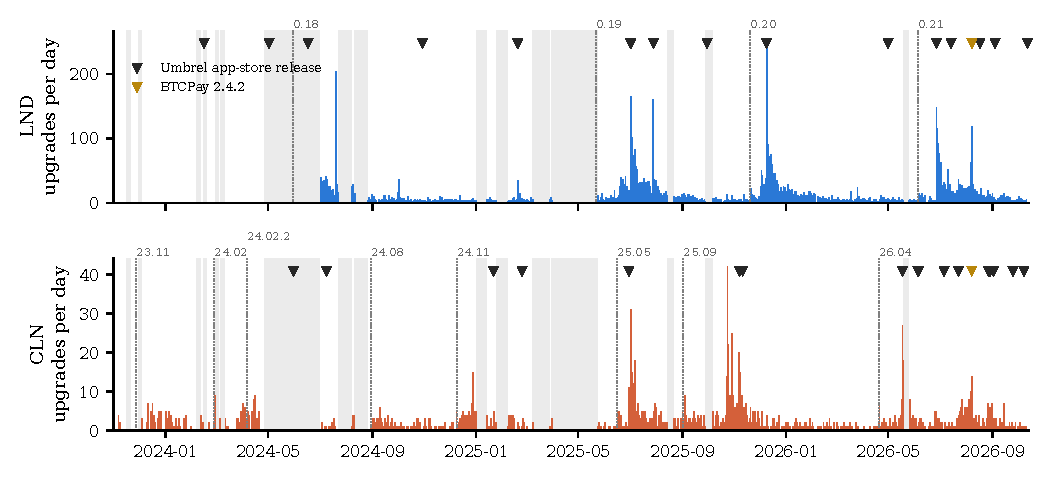
\includegraphics[width=\textwidth]{figures/fig5_waves.pdf}
\caption{Nodes first seen on a newer release line per day, where the upgrade day is known to within two days
(managed fleet excluded). Grey: snapshot gaps; dotted lines: LND and CLN releases; triangles: Umbrel app-store
releases (black) and BTCPay Server's security release 2.4.2 (gold) of that implementation.}
\label{fig:waves}
\end{figure*}

\subsection{Beyond the waves}
Platform releases account for a share of upgrades out of proportion to the time they cover. Since June~2025,
\PlatShareLND\% of LND upgrades whose day is known to within two days were signed within 48~hours after a platform
release that ships the new line, although these windows cover \PlatTimeLND\% of the time; for CLN, \PlatShareCLN\%
against \PlatTimeCLN\%. Since the platforms we cannot date are left out, these shares are lower bounds. The pushes
also check the inference: the nodes that changed line right after a platform shipped a new LND line landed on the
line it shipped (\S\ref{sec:validation}).
